\documentclass[11pt]{article} %tamaño mínimo de letra 11pto.

\usepackage{siunitx}
\usepackage{caption}
\usepackage{subcaption}
\usepackage{cite}
\usepackage{graphicx} 
\usepackage[english]{babel} %Español 
\usepackage[utf8]{inputenc} %Para poder poner tildes
\usepackage{vmargin} %Para modificar los márgenes
\setmargins{2.5cm}{1.5cm}{16.5cm}{23.42cm}{10pt}{1cm}{0pt}{2cm}
%margen izquierdo, superior, anchura del texto, altura del texto, altura de los encabezados, espacio entre el texto y los encabezados, altura del pie de página, espacio entre el texto y el pie de página

\usepackage{multirow}
\usepackage[table,xcdraw]{xcolor} 

\begin{document}
%%%%%%Portada%%%%%%%
\begin{titlepage}
\centering
{ \bfseries \Large UNIVERSIDAD COMPLUTENSE DE MADRID}
\vspace{0.5cm}

{\bfseries  \Large FACULTAD DE CIENCIAS FÍSICAS} 
\vspace{1cm}

{\large DEPARTAMENTO DE ESTRUCTURA DE LA MATERIA, FÍSICA TÉRMICA Y ELECTRÓNICA}
\vspace{0.8cm}

%%%%Logo Complutense%%%%%
{
\includegraphics[width=0.35\textwidth]{figuras/logoUCM.png}} %Para ajustar la portada a una sola página se puede reducir el tamaño del logo
\vspace{0.8cm}

{\bfseries \Large TRABAJO DE FIN DE GRADO}
\vspace{15mm}

{\Large Código de TFG:  ETE20 } \vspace{5mm}

{\Large Imagen por Ultrasonidos}\vspace{5mm}

{\Large Ultrasound Imaging}\vspace{5mm}

{\Large Supervisor/es: Joaquín López Herraiz}\vspace{18mm} 

{\bfseries \LARGE Ignacio Ortega Alonso}\vspace{5mm} 

{\large Grado en Física}\vspace{5mm} 

{\large Curso acad\'emico 2020-2021}\vspace{5mm} 

{\large Convocatoria de junio}\vspace{5mm} 

\end{titlepage}
\newpage

{\bfseries \large B-line scoring and detection in lung ultrasound }\vspace{10mm} 

{\bfseries \large Abstract: }\vspace{5mm} 

Ultrasound imaging is a widely used technique with multiple medical and industrial applications. It is based on the emission of high-frequency sound waves and the reception of their returning echoes. Measuring time delays and changes in pressure amplitude of the received waves, the scanned object's structure and acoustical properties can be inferred. Despite their acoustical properties being unsuited for ultrasound imaging, lungs can also be examined with this technique. Certain artifacts known as B-lines which may appear in lung ultrasound are indicative of pneumonia and similar pathologies such as COVID-19. Therefore, it has now become relevant to find methods able of detecting these artifacts. In this work, using a collection of assessed lung scans a machine learning algorithm was designed to detect B-lines based on a scoring scale. The results could be improved with changes in the scoring system, better quality data and more complex models.
 
\vspace{1cm}

\newpage


% CONTENTS 

\tableofcontents
\newpage

% ISSUES
%\begin{itemize}
%\color{red}
%\item dispersion relation: phase velocity / group velocity
%\item kind of transducer used
%\end{itemize}

% INTRODUCTION
\normalsize
\textcolor{red}{*revisar menciones de figuras}
\section{Introduction}

\subsection{Motivation and context: what does all this have to do with Physics?}

\subsubsection{The broad topic: Medical Physics and Artificial Intelligence}
	
	% Medical Physics
	Medical Physics consists of every application of physical theories to medicine. Among them are all of the medical imaging techniques that are carried out in radiology units of hospitals in order to diagnose diseases, such as X-rays, computed tomography (CT), magnetic resonance imaging (MRI) or ultrasound (US), as well as positron emission tomography (PET), which belongs to the area of nuclear medicine. Furthermore, there are therapeutical applications too such as radiotherapy, which allows to treat tumors with the aid of ionizing radiation.
	
	% Artificial Intelligence
	Artificial Intelligence (AI) is an umbrella term that englobes all the models and algorithms designed by humans in order to solve certain problems. In recent years, AI and in particular deep learning - a subcategory of the earlier - have shown great performance in several areas, Medical Physics being one of them \cite{shen}. For instance, it has been possible to detect skin cancer \cite{esteva} and pneumonia from chest X-rays \cite{rajpurkar} with great accuracy thanks to AI. There is such an interest in these techniques that the number of published articles on these topics in medical physics journals has grown exponentially (see fig).
	
	
	\begin{figure}[h]
	\centering
	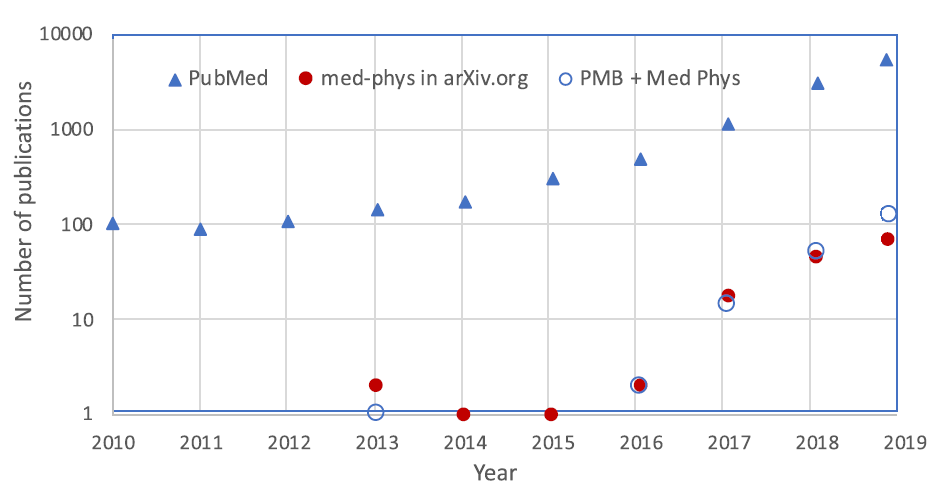
\includegraphics[width=0.6\textwidth]{figuras/DL_papers.png}	
	\caption{Número de publicaciones sobre IA y DL \cite{shen}}	
	\end{figure}
	
\subsubsection{The specific topic: Lung ultrasound and Covid-19}
	% Relevance of LUS in the Covid-19 pandemic context
	Recently, lung ultrasound (LUS) has become increasingly relevant due to the current situation of Covid-19 pandemic. Despite CT being the most established imaging technique for pneumonia monitoring and assessment, lung ultrasound advantages make it a promising tool to face this health crisis. First, ultrasound does use ionizing radiation, which makes it a suitable technique for pregnant women and children. In addition, it can be used in emergency and intensive care units without the need to take patients to the radiology unit, thus reducing the risk of infection and the workload for healthcare workers \cite{allinovi}. Lastly, diagnosis of Covid-19 with lung ultrasound has been proven to be comparable in accuracy to the CT standard \cite{ottaviani}.
	

	% Applications of AI to LUS
	Similarly to other fields of medical physics, lung ultrasound too has the potential for promising applications of AI. In particular, regarding lung ultrasound it is of great importance to correctly identify certain artifacts known as B-lines (see section x), whose presence is linked to different diseases, Covid-19 being one of them. An algorithm able to detect such artifacts would have multiple advantages: it would aid in the training of less experienced physicians, it could assist doctors in the diagnosis and it would speed up patient inspection times. Several of this type of algorithms have already been accomplished, both with the help of neural network classifiers \cite{vanSloun}\cite{born2020pocovid}\cite{cristiana2020automated}\cite{roy2020deep} and with more traditional algorithmic approaches \cite{brattain}\cite{moshavegh}.
	
	
\subsection{Physics of ultrasound imaging}
\subsubsection{Physical principles of ultrasound imaging}

	%(Overview)

	Medical ultrasound allows to obtain images of different body tissues thanks to the controlled emission of high-frequency sound waves and the reception of their reflections. Ultrasound probes are equipped with piezoelectric transducers that vibrate when excited with high-voltage electric pulses. This vibration is then transmitted through the body as a pressure wave whose behaviour is influenced by the mechanical properties of the tissues. A fraction of the energy emitted by the probe is reflected on tissue interfaces and received by the transducers. The transducers then vibrate and produce an electric signal that is processed in order to create an image of the examined region. 
	
	%(Sound as a wave)
	
	Sound waves can be understood as periodic variations of pressure on a propagation medium. The rate at which the pressure varies (frequency $f$) and the spatial distance between neighbouring points with equal pressure (wavelength $\lambda$) are related through the speed of sound $c = \lambda f$. The speed of sound $c$ depends on the elastic properties of the propagation medium, and it can be expressed as a function of bulk modulus $B$ and density $\rho$ by:
	
	\[  c = \sqrt{ \frac{B}{\rho} } \]
	
	In soft tissue, sound travels at an average speed of $ 1540 \si{\meter\per\second} $, but it can be as slow as $ 600 \si{\meter\per\second} $ in the lungs, or as fast as $ 3200 \si{\meter\per\second} $ in bones (see table 1). 
	
	%(Reflection and acoustic impedance)
	
	Another property of a medium which is related to the speed of sound is acoustic impedance, defined as: 	
	
	\[ Z = \rho c \]
	 	
	Differences in acoustic impedances of adjacent tissues are responsible for the reflection of sound waves. More exactly, the ratio between the pressure amplitudes of the reflected ($P_r$) and incident ($P_i$) wave can be expressed as	
	
	\[ \frac{P_r}{P_i} = \frac{Z_2 – Z_1}{Z_2 + Z_1} \]	
	
	where $Z_1, Z_2$ are the acoustic impedances of the proximal and distal tissues respectively. An intensity reflection coefficient can also be defined as: 	
	
	\[ R_I = \frac{I_r}{I_i} = \left( \frac{P_r}{P_i} \right)^2 \]	
	
	making use of the fact that intensity is proportional to the squared power of pressure amplitude. For some interfaces like fat-muscle this coefficient is very small, meaning that most of the energy carried by the wave keeps propagating. For others, such as muscle-air almost all the energy is reflected.

	%(Scattering)
	
	When the size of the objects responsible for reflection is similar or smaller than the wavelength, sound is reflected in all directions or scattered. The amount of scattered energy depends on acoustic impedance differences, but also on the texture of the tissue and the wavelength.

	%(Attenuation)
	
	Scattering, together with tissue absorption, are responsible for the attenuation or loss of energy of the propagating waves. Different tissues have different attenuation coefficients. They are typically measured in units of $dB/cm$ and are proportional to frequency. In other words, waves with longer wavelength can penetrate deeper into the body. \cite{bushberg}

\begin{table}[]
\centering
\begin{tabular}{l|l|l|l|l}
            & $  \rho (kg  \cdot m^{-3})$ & $c (m \cdot s^{-1})$ & $Z (kg \cdot m^{-2} \cdot s^{-1})$ &  \\ \cline{1-4}
Air         & $1.2$                       & $330$                & $400$                              &  \\
Lung        & $300$                       & $600$                & $1.8 \cdot 10^5$                   &  \\
Soft tissue & $1050$                      & $1540$               & $1.6 \cdot 10^6$                   &  \\
Bone        & $1650$                      & $3200$               & $5.3 \cdot 10^6$                   & 
\end{tabular}
\caption{Typical values of density, speed of sound and acoustical impedance \cite{farr}}
\end{table}


\subsubsection{Transducers, beam properties}

	%(Transducers)

	Ultrasound waves are produced by transducers made of piezoelectric materials. Because of the way electric dipoles are arranged in this kind of materials, they vibrate when a voltage difference is applied to their surfaces. Similarly, when an external force makes them contract or expand, a difference in voltage appears between their surfaces. This property allows them to operate both as transmitters and receivers of sound waves. An important property of a transducer is its Q factor, which is defined as: \[ Q = \frac{f_0}{\Delta f} \] where $f_0$ is the resonant frequency of the transducer and $ \Delta f$ is its bandwith, that is, the range of frequencies around $f_0$ where energy is also emitted. These frequencies are introduced by dampening the vibration of the piezoelectric and thus making the emitted pulse shorter. Transducers that are lightly damped show a  narrow bandwith (high Q factor) and a long spatial pulse length, whereas heavily damped transducers have broad bandwiths (low Q factor) and short spatial pulse length (figure 1). 

	\begin{figure}
	\centering
		\begin{subfigure}{0.49\textwidth}
		\centering
		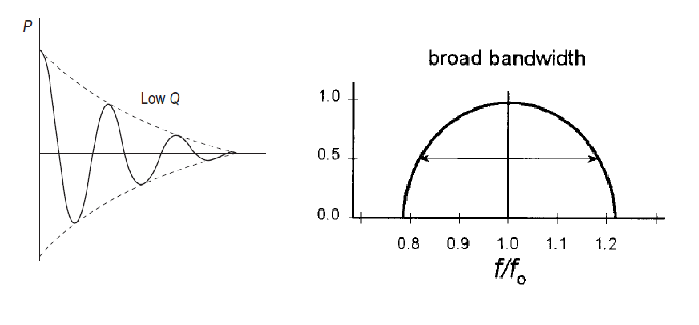
\includegraphics[width=\textwidth]{figuras/lowq.png}
		\caption{Low Q, broad bandwith, short pulse}
		\end{subfigure}
		\centering
		\begin{subfigure}{0.49\textwidth}
		\centering
		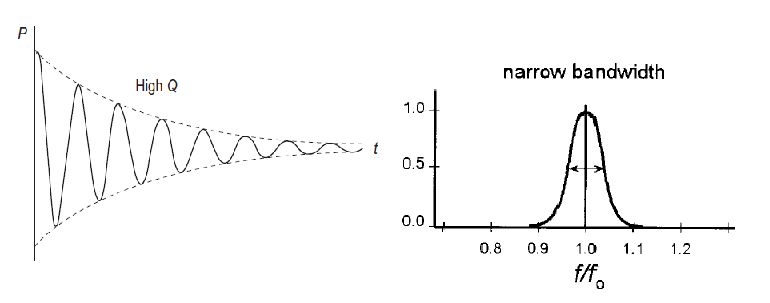
\includegraphics[width=\textwidth]{figuras/highq.png}
		\caption{High Q, narrow bandwith, long pulse}
		\end{subfigure}	
	\caption{Low Q and high Q: spectrum and pulse comparison\cite{bushberg}\cite{farr}}	
	\end{figure}

	%(Near and far field)
	
	Several piezoelectric elements are arranged in transducer arrays and operate together to produce an ultrasound beam. The shape of the beam is the result of interference between every individual emitter. It is characterized by two regions: a near field where the beam is converges and a far field where it diverges. The length of the near field (or in other words, the focal distance) is related to the effective diameter of the transducer and its frequency by: \[ l \propto \frac{d^2}{\lambda} \] That is, wider transducers and higher frequencies produce longer focal distance.

	%(Spatial resolution)
	
	The ability to resolve objects in the acquired image is determined by a series of parameters of the beam and transducers. In the axial direction (direction of the beam), resolution is limited by the spatial pulse length (SPL). Two returning echoes can only be resolved if the distance between them is greater than the SPL. Therefore, for two reflectors to be distinguished they cannot be separated by a distance greater than half the SPL (figure 2). Shorter SPL can be achieved with shorter wavelength or fewer cycles per pulse, i.e. lower Q factor. Typical axial resolution values are of $0.5 mm$. Because SPL is constant along the beam, axial resolution is independent of depth.
In the perpendicular direction resolution is determined by the diameter of the beam. For this reason lateral resolution is best at the focal zone and it decreases in the near and far fields. Some transducer arrays can produce beams of variable focal distance, creating an extended focal zone where lateral resolution is optimal. 

	\begin{figure}
	\centering
	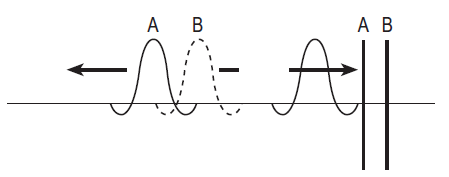
\includegraphics[width=10cm]{figuras/resolution.png}
	\caption{\color{red} (no se entiende bien, dividir en dos) Axial resolution: separation between reflectors A and B must be must 		be smaller than $\frac{1}{2} SPL$ \cite{farr}}
	\end{figure}


\subsubsection{Image formation}
	
	In order to generate a two-dimensional ultrasound image several steps have to be followed. First transducers are set to 'transmit mode' to produce sound pulses using a high voltage spike. After the pulse is emitted, they are set to 'receive mode' in order to capture vibrations of returning echoes. Echoes received earlier correspond to reflections taking place close to the transducer, while later echoes are produced by deeper reflectors.  The returning echoes are very weak and can only induce small voltages in the transducers that need to be amplified. In addition, later echoes are significantly weaker than earlier ones due to attenuation experienced by the sound wave throughout its round-trip. To compensate for this an additional time-dependent amplification known as time gain compensation (TGC) is introduced. The outcome of this process is a signal containing information of the scanned tissues along the beam direction, where amplitude is proportional to acoustic impedance differences and time corresponds to depth. Assuming an average speed of sound of $1540 m/s$ along the beam path, time and depth are related through \[ D = \frac{c·t}{2} \] where the 2 factor accounts for the round-trip distance. After a certain time interval, transducers are set to emit the next pulse and the whole process is repeated several times per second with different focus parameters to achieve a two-dimensional image. 

\subsubsection{Lung Ultrasound and artifacts}

	%(Artifacts)

	As with any other imaging device, ultrasound cannot reproduce anatomy with unlimited accuracy. Artifacts are deviations from the actual aspect of the scanned objects due to the intrinsic working principles of the device. Lungs are particularly prone to exhibit artifacts when probed with ultrasound, but valuable information can still be obtained from its examination when the origin of these artifacts is well understood. A typical lung ultrasound image shows the following features. First, a very bright and approximately horizontal line can be seen in the upper half of the picture, corresponding to the pleura. The pleura is a thin membrane inside the chest cavity where lungs are contained. When probing perpendicular to the ribs, these can be also seen as dark regions above the pleura projecting shadows downwards. Due to the high difference of acoustic impedance between the soft tissue above the pleura and the air-filled lung below it, almost all the energy carried by sound waves is reflected, making observation of deeper tissues impossible. A common artifact that can be observed in the region below the pleural line is A-lines (figure 3.b). A-lines appear like equally distanced bright lines parallel to the pleural line and they can be explained as a reverberation artifact. Due to the high reflectivity of the pleura, echoes can bounce back and forth several times between it and the transducer surface (figure 3.a). Because of their delay with respect to the emitted pulse, these echoes are interpreted as multiple objects located further away from the transducer \cite{artifacts}.

	%(B-lines)
	
	Another reverberation artifact that can be commonly observed in lung ultrasound is B-lines (figure 3.c). Whereas A-lines are usually present in healthy lungs, B-lines are correlated with interstitial syndrome, a kind of disease where inflammation or acummulation of fluid makes thin tissues within the lung called interstitium to thicken. This can be observed for example in pneumonia patients. While the exact origin of this artifact is not clearly understood, it is thought that it is originated from reverberation between closely located high reflective surfaces, like air-liquid. Because of the proximity between reflectors the resulting echoes are not distinct, but rather appear as a bright and diffuse vertical line stretching from the pleural line downwards. During the current pandemic, lung ultrasound has proved to be a reliable method for diagnostic and monitoring of Covid-19 pneumonia through the assessment of B-lines and similar phenomena.
	
	\begin{figure}
	\centering
		\begin{subfigure}{0.25\textwidth}
		\centering
		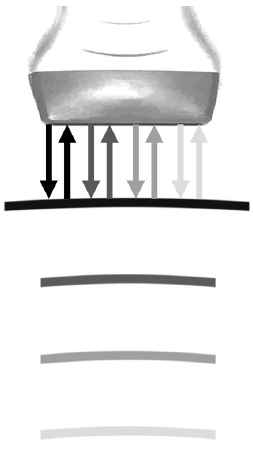
\includegraphics[width=\textwidth]{figuras/reverberation.png}
		\caption{Reverberation artifact}
		\end{subfigure}	
		\begin{subfigure}{0.3\textwidth}
		\centering
		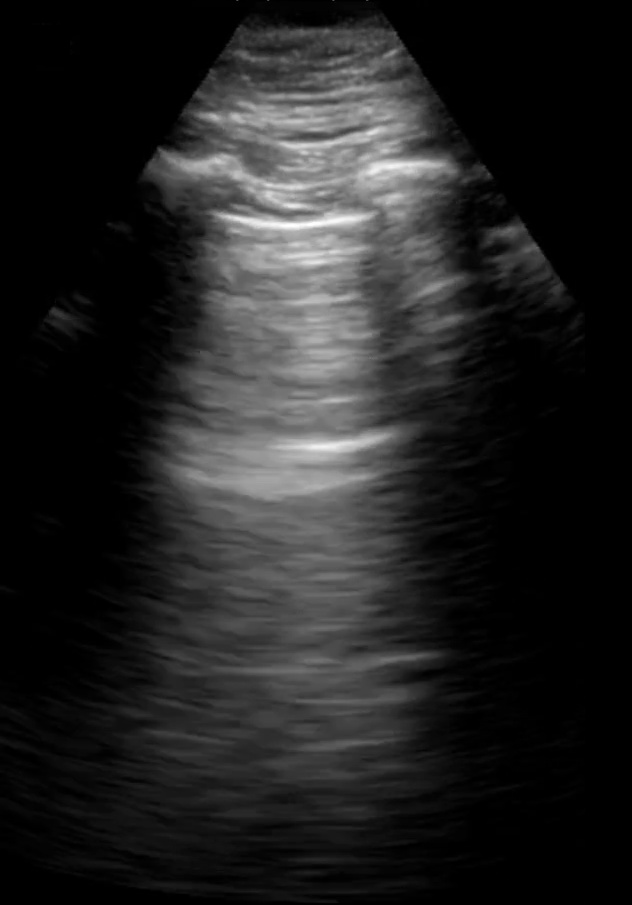
\includegraphics[width=\textwidth]{figuras/alines.jpg}
		\caption{A-lines}
		\end{subfigure}
		\centering
		\begin{subfigure}{0.3\textwidth}
		\centering
		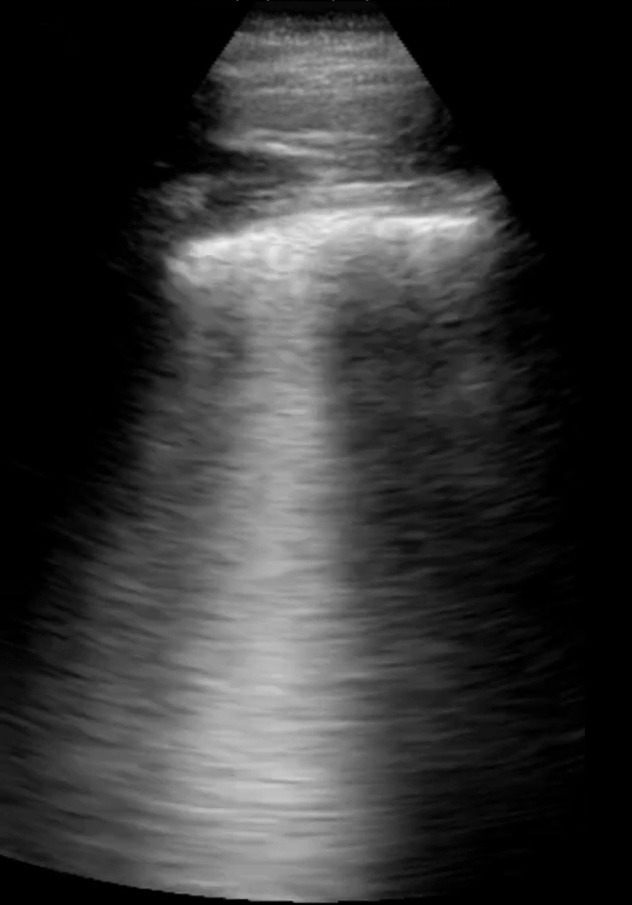
\includegraphics[width=\textwidth]{figuras/blines.jpg}
		\caption{B-lines}
		\end{subfigure}	
	\caption{\color{red} (cambiar figura) Common ultrasound artifacts found in lungs}	
	\end{figure}
	%(Artificial Intelligence)
	


\section{Objectives}

	The present work explores a particular topic from different perspectives and with different goals.

	Firstly, it focuses on understanding ultrasound imaging from a theoretical point of view. It aims to identify the physical principles that rule its operation, as well as explaining the image artifacts that are characteristic of this technique. In particular, those artifacts present in lung ultrasound are explored.
	
	Secondly, the current state of research on the topic in question is explored in the scientific literature. Besides considering the broader context of medical physics to which the topic belongs to, emphasis is placed on recent applications of artificial intelligence to lung ultrasound.

	Apart from that, this work also gathers the outcome of a collaboration with Ultracov project, with the aim to have a first experience in research.

	Lastly, a practical approach has also been taken on the topic under discussion in order to become familiarised with a programming language and other tools. An analysis of a collection of lung ultrasound videos has been carried out, and its results have been interpreted. 
	
	
	
% MÉTODOS
\section{Methods}

\subsection{Software tools}
	Different tools have been used throughout the project. Python programming language has been chosen to perform the analysis on the videos due to its popularity among the scientific community and the wide offer of libraries available. These are collections of pre-written and documented code designed for different purposes: numpy for matrix and numerical calculations, matplotlib for graphs and visualizations, openCV for image analysis and scikit-learn for machine learning algorithms, among others.

	Once we have all the necessary libraries to develope our algorithms, we need an application to edit our code, test it and debug it: this is the role of an integrated development environment (IDE). Both Sypder and PyCharm have been used.
	
	Finally, it is also useful to have some way of organising our code and handling updates. To this purpose, version control applications such as GitHub are of great help. They allow developers to save their source code online and keep track of any changes or updates. It is specially useful when collaborating with other developers.


\subsection{Dataset}

	In order to train our model we have made use of a collection of 280 ultrasound videos of lungs. The videos correspond to a single patient throughout a 40 day period of regular examinations monitoring the evolution of Covid-19 pneumonia. They were taken and labelled according to B-lines presence by an experienced physician (Dr. Yale Tung Chen \cite{tung2020lung}
	 - Hospital Universitario Puerta del Hierro) as part of the ULTRACOV project. All videos were taken with a Butterfly iQ probe with settings of scan depth ranging from 7 cm to 14 cm. Most of the scans belong to regions of the chest where lung is the only visible organ, but on a total of 78 videos other organs such as liver or spleen show up. An image resolution of 1080$\times$632 pixels and framerate of 21 fps is constant across the whole database. Video durations vary widely, ranging from 1 second to 20 seconds of length, with an average of 6 seconds per video. 
	
	Each video was labelled depending on whether B-lines were present or not at any instant throughout the video. In other words, videos labelled as 'no B-lines' do not exhibit them on any of their frames whereas videos labelled as 'B-lines' do, at least on a fraction of their frames but not necessarily in all of them. This is due to the natural motion of the lungs while breathing, as well as motion of the probe and changes in direction of observation. Because of this, it is necessary to  separate videos in smaller sections and isolate those corresponding to B-lines presence. A total number of 93 videos out of 280 are labelled as 'B-lines', which adds up to a $33 \%$ frequency of occurrence. 
	
	The frames making up each video were extracted on separate directories and cropped to remove unnecessary details for the later analysis. As a result, a collection of gray-scaled images sized 905$\times$632 pixels and 8 bits of depth (i.e., brightness values ranging from 0 to 255) was obtained.

	 
\subsection{Polar format of ultrasound images}

	Computing 3 cluster centroids per video greatly simplified the original dataset to a collection of images where each video is represented by three images. Before performing any analysis on the samples we have to make our dataset as homogeneous as possible. Once every video has been narrowed down to three images regardless of its duration, there are still differences across samples with respect to their maximum scan depth. These differences manifest themselves as changing aperture angles of the circular sector shapes of the images. Images with a shallower scan range show a wider aperture angle while those with a deeper range show narrower angles. In order to make these differences less apparent across the dataset we perform a reshaping of the images to a 'polar coordinates' format. To achieve this, we first manually measured the aperture angle on the image for each scan depth value (7, 8, 9, 10, 13 and 14 cm). Next, we divided the circular sector into several regions of equal radial and angular coordinates (figure 6.a). Finally, we took the mean value of brightness on each region and assigned it to the reshaped image (figure 6.b). By doing so, we obtained a rectangular-shaped image of N-rows by M-columns. In particular, we have chosen $N = M = 50$ (figure 6.c).
	
	This reshaping of the images also facilitates further calculations, as we have greatly reduced the size of the images. It also helps identify B-lines more easily, as they should now appear as vertical lines whereas originally they could take diagonal shapes. 
	
	\begin{figure}
	\centering
		\begin{subfigure}{0.29\textwidth}
%		\centering
		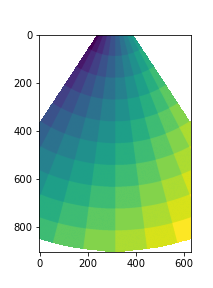
\includegraphics[width=\textwidth]{figuras/polar_original.png}
		\caption{}
		\end{subfigure}
%		\hfill
		\begin{subfigure}{0.35\textwidth}
%		\centering
		
\includegraphics[width=\textwidth]{figuras/polar_new.png}
		\caption{}
		\end{subfigure}
%		\hfill
		\begin{subfigure}{0.30\textwidth}
%		\centering
		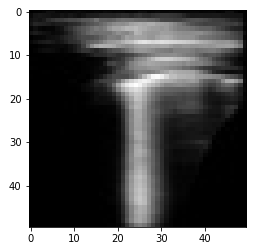
\includegraphics[width=\textwidth]{figuras/polar.png}
		\caption{}
		\end{subfigure}
	\caption{Reshaping of images into polar coordinates}
	\end{figure}	
	
	
\subsection{Frame-based clustering of ultrasound videos}

	Following the extraction and cropping of frames, every image set corresponding to a a video has to be divided into smaller sets in order to simplify the analysis and isolate potential B-lines. To achieve this, a K-means clustering algorithm implemented in the Scikit-learn toolkit was used \cite{sklearn}. Clustering algorithms are a kind of unsupervised learning algorithms whose aim is to subdivide a dataset into separate groups or clusters in such a way that data points belonging to the same cluster are as close as possible to each other. K-means is one of the simplest of these algorithms. When applied to a two-dimensional dataset the result looks like the following (figure 4)\cite{python}. Each cluster is represented by a cluster center or 'centroid', which corresponds to the average of the data points belonging to that cluster. Each data point is assigned to the cluster whose centroid is the closest. Different configurations are computed one after another until the total sum of distances within clusters is minimized, also known as 'inertia' parameter:
	
	\[ I = \sum_j^N \sum_{x_i \in C_j} || \vec{x_i} - \vec{ \mu_j} ||^2 \]
	
	where $N$ is the total number of clusters, $\vec{\mu_j}$ is the 'centroid' of the j-th cluster $C_j$ and $\vec{x_i}$ are data points.
	
	When working with images, instead of two dimensions each data point $\vec{x_i}$ belongs to an n-dimensional space with n being equal to the number of pixels in the image ($905 \times 632=571960$ in our case). The resulting cluster centroids can be reshaped to the original dimensions to obtain averaged images of each cluster of frames. For every video in our collection three clusters have been computed with the purpose of obtaining a simplified representation of the video and isolating fragments of it that may exhibit B-lines (figure 5). 
	
	\begin{figure}
	\centering
	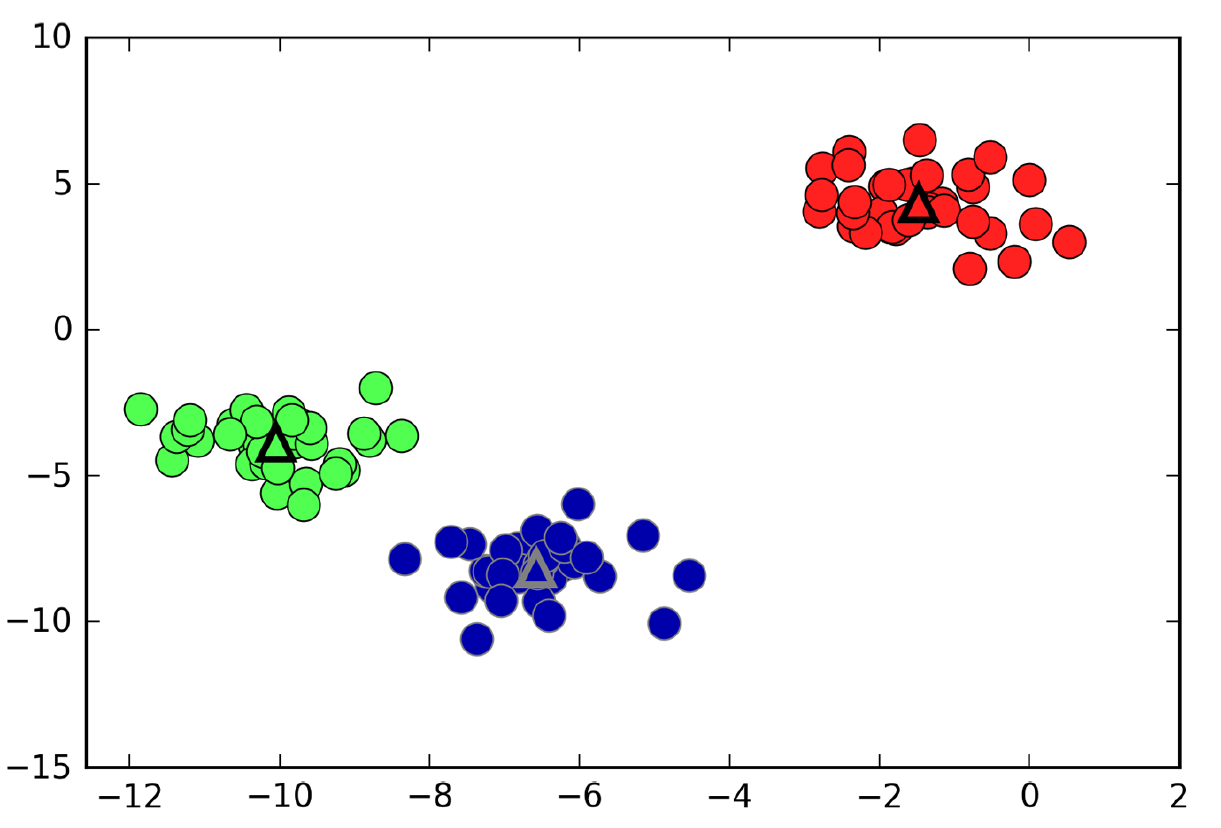
\includegraphics[width=10cm]{figuras/clusters.png}
	\caption{K-Means: each cluster (red, green, blue) is represented by its centroid (triangles)\cite{python}}
	\end{figure}
	
	\begin{figure}
	\centering
		\begin{subfigure}{0.3\textwidth}
		\centering
		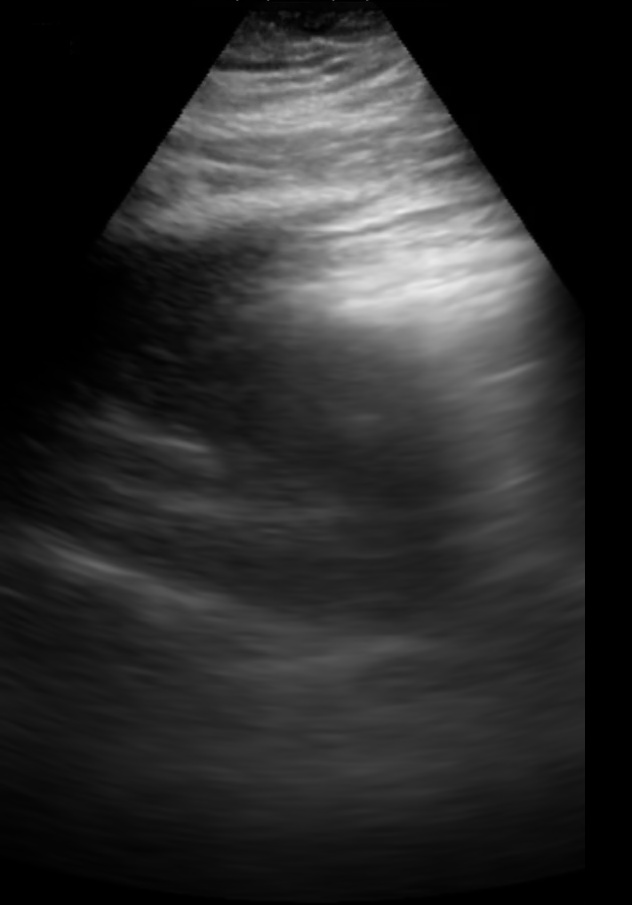
\includegraphics[width=\textwidth]{figuras/centroid_0.jpg}
		\end{subfigure}
		\begin{subfigure}{0.3\textwidth}
		\centering
		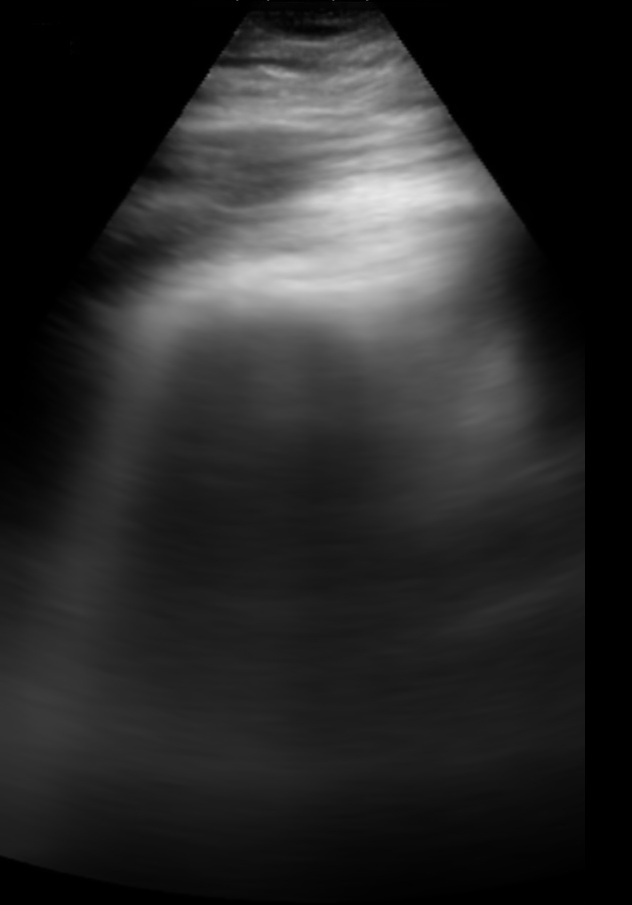
\includegraphics[width=\textwidth]{figuras/centroid_1.jpg}
		\end{subfigure}
		\begin{subfigure}{0.3\textwidth}
		\centering
		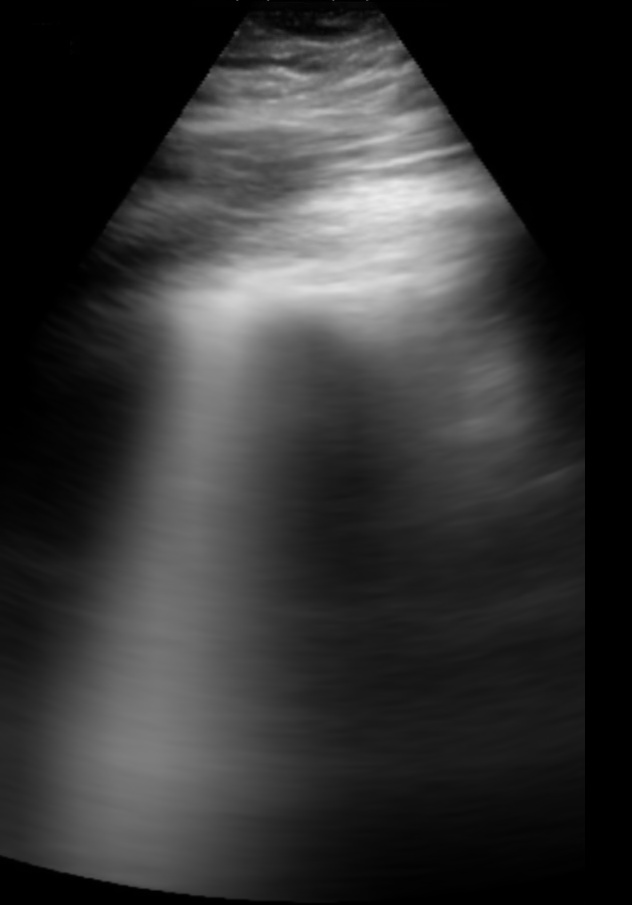
\includegraphics[width=\textwidth]{figuras/centroid_2.jpg}
		\end{subfigure}
	\caption{\color{red} (explicar mejor) A set of three centroids representing clusters of frames of a single 		video}
	\end{figure}

	

\subsection{B-line scoring (*feature extraction from ultrasound images)}

	We now describe a scoring system used to evaluate the likeliness of an image to show B-lines. Such a scoring system must take into account known features of B-line pattern: bright, uniform vertical shapes extending from the pleural line to the lower margin of the image. Images exhibiting B-lines should generate high scores on this scale, whereas those who show none should produce lower scores. The final score of a video is taken as the maximum score of all of its three centroids. All scorings are performed on the images in polar format. In this work three scoring scales have been used:
	
\begin{itemize}
	\item \textbf{Total mean brightness}: average intensity is calculated for every column on the image. The highest value obtained is chosen as the outcome. Values are normalized to the peak brightness of the image.
	\item \textbf{Lower quarter mean brightness}: average intensity is calculated for every column on the quarter section that is further away from the transducer. This should highlight the fact that B-lines extend down to the lowest margin of the image, while other artifacts fade away faster. Values are normalized to the peak brightness of the image.
	\item \textbf{Fraction of column above half-maximum}: maximum brightness is calculated across every column. Next, the number of pixels with intensity above half of this value is counted on every column, and its ratio to the total length of the column is taken as the outcome. 
\end{itemize}

Once scored, every video should yield a set of three values corresponding to each scoring scale. All values are in the range $[0,1]$ due to the normalization chosen. It is important to note that other scoring systems could be used. The one we present has been chosen because of its simplicity and easy interpretation.

\subsection{Image classification with logistic regression}

	If our scoring system correlates well with the presence of B-lines, we should be able to train a machine learning algorithm that is able to predict the presence or absence of B-lines in a video based on its score. We have chosen a logistic regression implementation in Scikit-learn toolkit \cite{sklearn}. Logistic regression is a kind of supervised learning algorithm that assigns a data point to a class where it is most probable to belong to. It takes advantage of logistic functions, also known as sigmoids, by taking a continuous variable as an input and yielding a probability value between 0 and 1 as output. 

	\[ f(x) = \frac{1}{1+ e^{-x}} \]
	
	Probabilities below or above 0.5 correspond to one or the other class. The value of the input variable corresponding to a probability of 0.5 is known as the decision boundary (figure 7). In this case, three values per sample are fed to the algorithm as input, corresponding to each scoring scale, and two different values make up the output, corresponding to the probabilities of presence or absence of B-lines.
	
	\begin{figure}
	\centering
	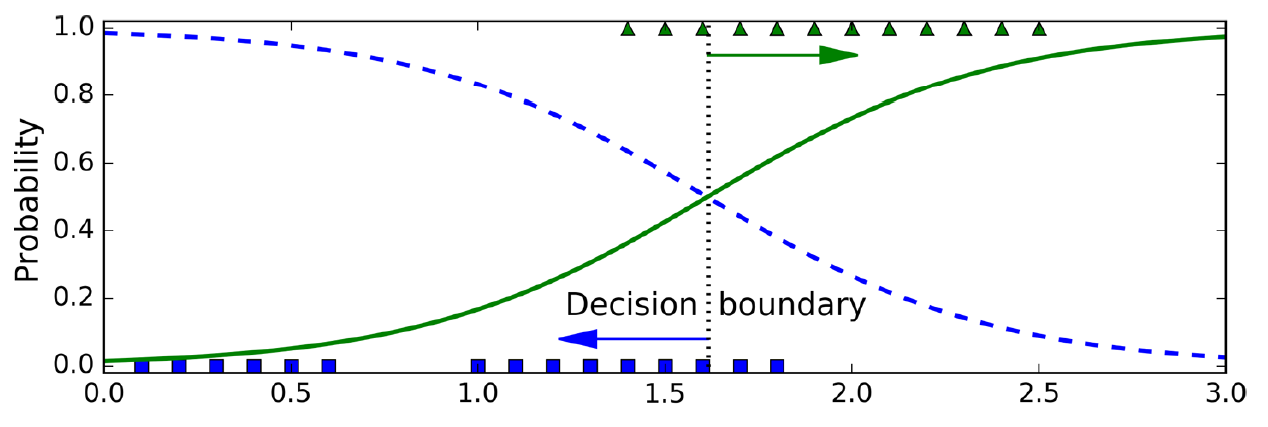
\includegraphics[width=11cm]{figuras/sigmoid.png}
	\caption{Example of a logistic function fit to a set of data. Values above the decision boundary are assigned to class 1. \cite{geron}}
	\end{figure}


% RESULTADOS
\section{Results}

\subsection{ULTRACOV project}
	As part of this work a collaboration with Ultracov project has also been made. Ultracov project aims to develop an ultrasound device specific for Covid-19 detection. To this purpose, different AI algorithms are being developed. As our contribution to the project, we have gathered these tools and integrated them in a graphical user interface (GUI) using Python and the PySimpleGUI library. The GUI also allows to display videos and manually assign labels to them based on the anomalies that they show, in order to calculate a score of lung involvement. 
	The following tools have been included:
	\begin{itemize}
	\item Motion detection: it provides a graph of the lateral displacement in pixels of the video through an optical flow algorithm.
	\item Pleura detection: it shows the predicted location of the pleural line on the current video using a pre-trained neural network.
	\item Similar images: it displays a selection of the most similar images to the current one from a dataset.
	\item Image quality: it analyses whether the probe is properly placed based on the pleura detection tool (if no pleura can be seen the quality is not good).
	\end{itemize}
	
	\begin{figure}
	\centering
	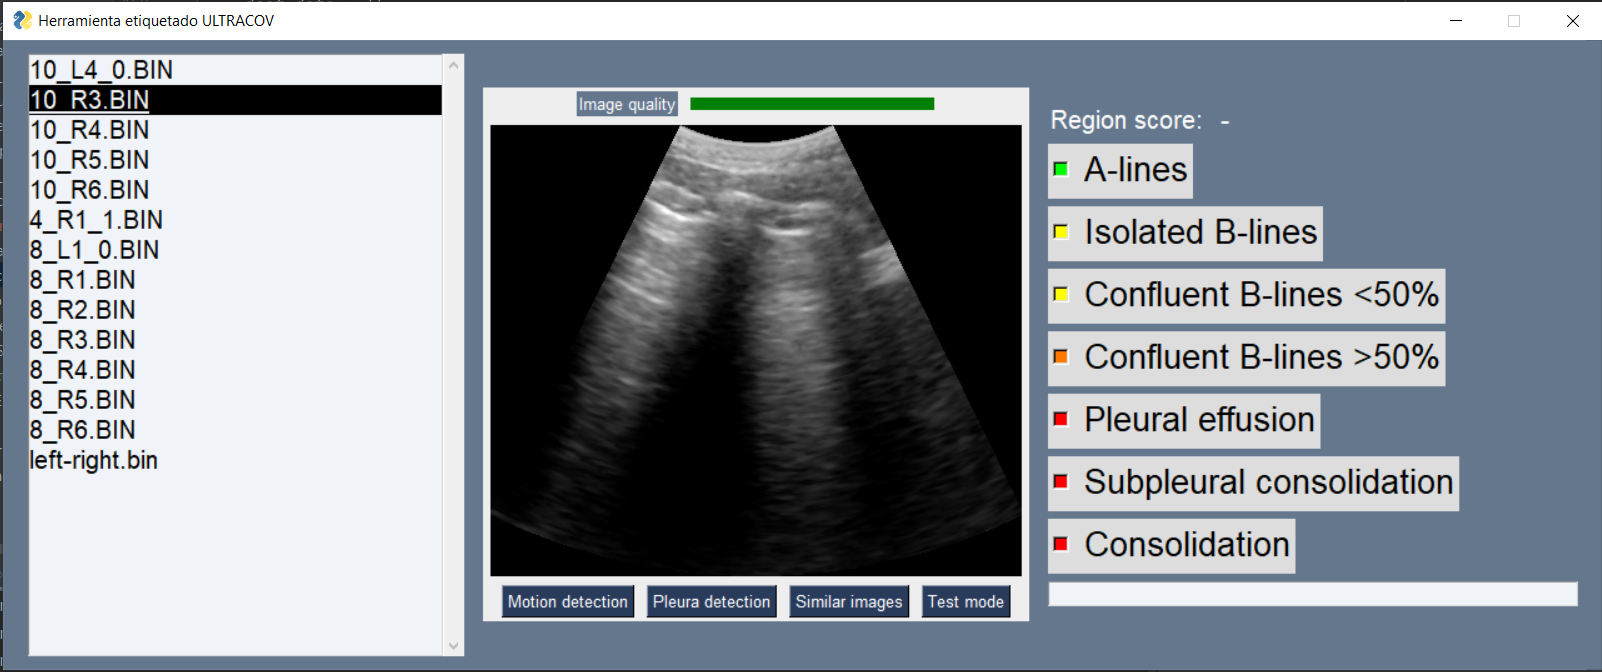
\includegraphics[width=0.8\textwidth]{figuras/ultracov_GUI.png}
	\caption{Graphical user interface including analysis tools for Ultracov project.}
	\end{figure}
	
	
\subsection{Video analysis}

	Before training the logistic regression algorithm, our dataset has been split into two different sets. The first one is the training set, i.e. the collection of labelled videos that will be fed to the algorithm. The second one is the test set, on which the algorithm's prediction will be evaluated. Ratios of 0.8 and 0.2  out of the total dataset have been chosen respectively for the training and test sets. In other words, the algorithm is trained on 224 out of the total 280 samples, and it is tested on the remaining 56 samples. Both subsets must contain a similiar ratio of samples labelled as B-lines as in the original dataset in order to remain representative (figure 8). 
	
	\begin{figure}
	\centering
	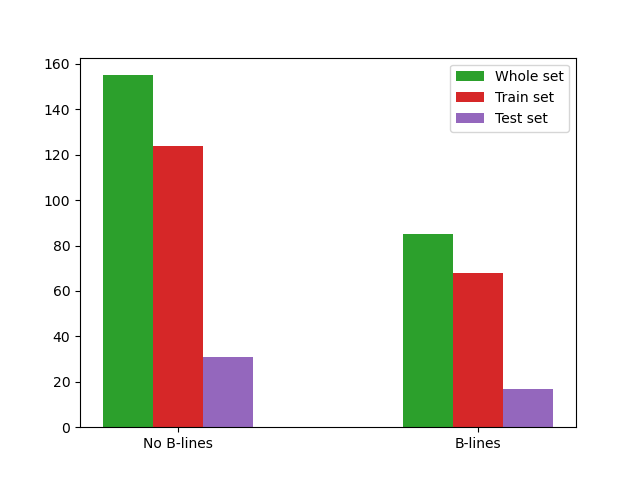
\includegraphics[width=0.5\textwidth]{figuras/bline_ratio.png}
	\caption{B-lines/no B-lines ratio of occurrence must be constant across all 		sets}
	\end{figure}

	\begin{figure}
	\centering
		\begin{subfigure}{0.65\textwidth}
		\centering
		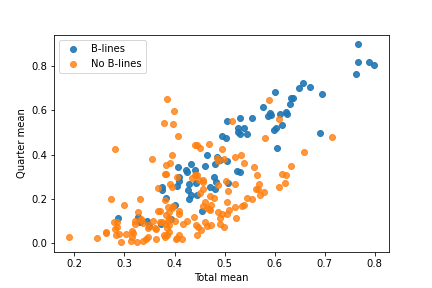
\includegraphics[width=\textwidth]{figuras/scores1_2.png}
		\caption{Lower quarter mean brightness against total mean brightnes}
		\end{subfigure}

		\begin{subfigure}{0.65\textwidth}
		\centering
		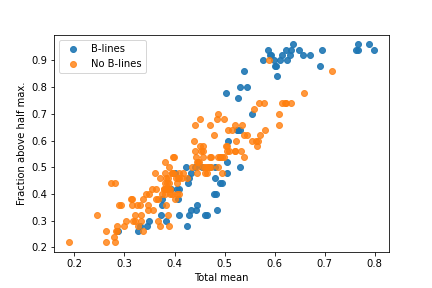
\includegraphics[width=\textwidth]{figuras/scores1_3.png}
		\caption{Fraction above half-max against total mean brightnes}
		\end{subfigure}

		\begin{subfigure}{0.65\textwidth}
		\centering
		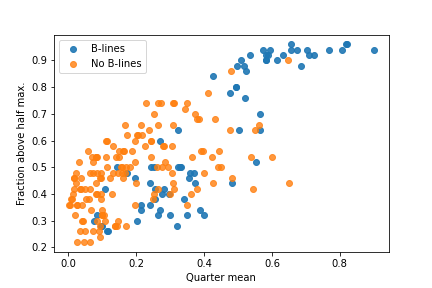
\includegraphics[width=\textwidth]{figuras/scores2_3.png}
		\caption{Fraction above half-max against lower quarter mean brightness}
		\end{subfigure}
	
	\caption{Score distribution of the training dataset in all combinations of the 	three scoring scales. True labels are shown (B-lines / no B-lines)}
	\end{figure}

	Scores of all videos in the training set have been calculated and represented  against each other in figure 9. All of the three scoring scales are approximately correlated, as expected. That means that those videos who score high in one scoring scale also show high scores in the other scales, i.e. the scoring system is coherent. However, there is much overlap among scores of videos which show B-lines and those which do not. In other words, in this representation there is not a clear boundary between each class of data points. 
	
	A comparison between the algorithm's prediction and the true values is summarized in table 1 in what is known as a 'confusion matrix'. Elements in the diagonal of the matrix are correct predictions (true positives or true negatives), while elements out of the diagonal are wrong predictions (false positives or false negatives).  The accuracy of the prediction is defined as the total ratio of correct predictions: 
	
	\[ ACC = \frac{TP + TN}{TP + TN + FP + FN}	\]
	
	With 39 correct predictions out of 56 samples the accuracy of the algorithm is $ACC = 70 \%$. 
	
	The ratio of correctly identified positives is measured by sensitivity or 'true positive rate' (TPR) and it is defined as:
	
	\[ TPR = \frac{TP}{TP + FN} \]
	
	With only 5 predicted B-lines out of the existing 19, the achieved sensitivity is $ TPR = 26 \% $.

	Conversely, the amount of true negatives detected is measured by specificity or 'true negative rate' (TNR):
	
	\[ TNR = \frac{TN}{TN + FP} \]
	
	which in our case sums $ TNR = 92\%$, with 34 out of 37 detected.
	
	Finally, precision or 'positive predictive value' (PPV) is defined as the ratio of true positives to all predicted positives:
	
	\[ 	PPV = \frac{TP}{TP + FP} \]
	
	 Of a total of 8 predictions of B-lines, 5 are true positives, which implies a precision of $ PPV = 63\% $.
	

\begin{table}[]
\centering
\begin{tabular}{cccc}
\multicolumn{2}{c}{}                                                                & \multicolumn{2}{c}{Truth}                                                                                                                  \\ \cline{3-4} 
\multicolumn{2}{c}{\multirow{-2}{*}{}}                                              & \multicolumn{1}{c|}{B-lines}                             & \multicolumn{1}{c|}{No B-lines}                                                 \\ \cline{2-4} 
\multicolumn{1}{c|}{}                             & \multicolumn{1}{c|}{B-lines}    & \multicolumn{1}{c|}{\cellcolor[HTML]{3399FF}\textbf{5}}  & \multicolumn{1}{c|}{\cellcolor[HTML]{FF9933}\textit{3}}                         \\ \cline{2-4} 
\multicolumn{1}{c|}{\multirow{-2}{*}{Prediction}} & \multicolumn{1}{c|}{No B-lines} & \multicolumn{1}{c|}{\cellcolor[HTML]{3399FF}\textit{14}} & \multicolumn{1}{c|}{\cellcolor[HTML]{FF9933}{\color[HTML]{333333} \textbf{34}}} \\ \cline{2-4} 
\end{tabular}
\caption{Confusion matrix: (left to right, top to bottom) true positives (TP), false positives (FP), false negatives (FN), true negatives (TN).}
\end{table}
	
	\begin{figure}[h]
	\centering
	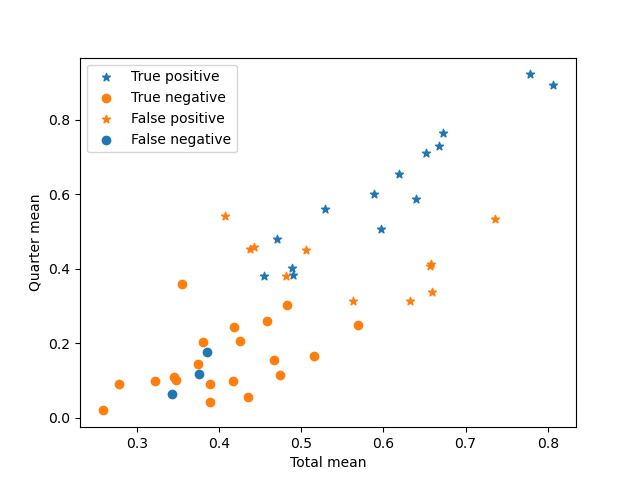
\includegraphics[width=11cm]{figuras/discussion.png}
	\caption{Score distribution and predictions on test set}
	\end{figure}	


% DISCUSIÓN Y CONLCUSIÓN
\section{Discussion}

	The proposed algorithm has shown a specificity of $92 \%$ in the identification of B-lines, meaning that very few false positives were produced. However, a sensitivity of only $26 \%$ has been achieved, implying a great number of false negatives.  This can be explained by the score distribution of the dataset (figure 9). It can be seen that there is a great overlap between data points belonging to different classes. Therefore, the algorithm cannot determine a clear boundary between them. This also explains the low accuracy obtained ($70\%$) compared to the original distribution of B-lines ($ 33\% / 66\%$). An algorithm that predicts every sample not to show B-lines would show an accuracy of $66\%$.
	
	
	There are different explanations for the overlap in the score distribution. On one hand, the source of error can be in the scoring system itself. For example, the 'quarter mean' scale may not always be indicative of B-lines. When organs such as the spleen appear on a video, the brightness on the lower half of the image increases (see figure 11.a) even if there are no B-lines. This could cause a false positive. 'Total mean brightness' and 'fraction above half maximum' may also induce false positives due to the high intensity region above the pleural line, specially on the short range images (figure 11.b). Therefore, changes on the scoring system could improve the accuracy of the algorithm.
	
	\begin{figure}[h]
	\centering
	\begin{subfigure}{0.4\textwidth}
	\centering
	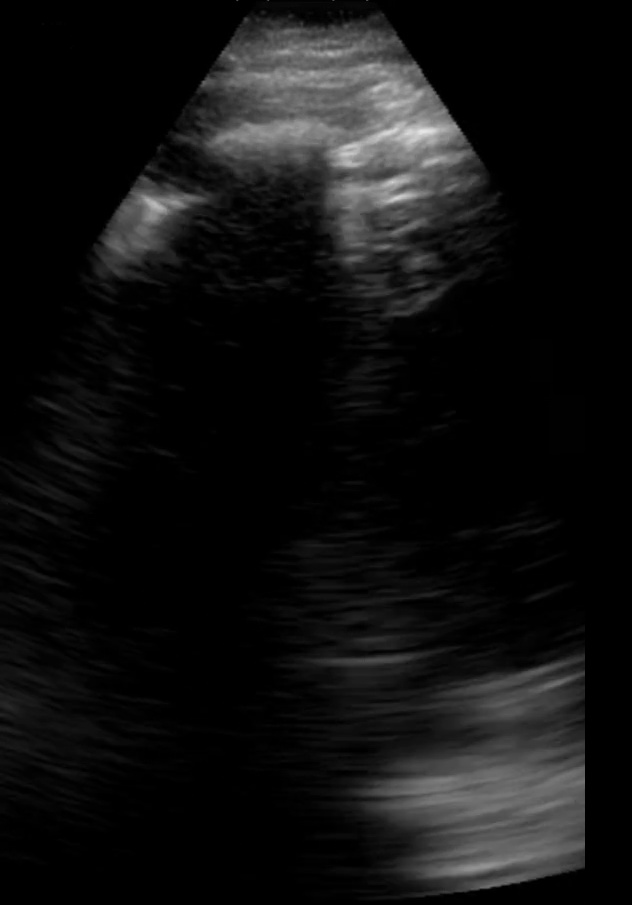
\includegraphics[height=6.5cm]{figuras/spleen.jpg}
	\caption{}
	\end{subfigure}
	\begin{subfigure}{0.4\textwidth}
	\centering
	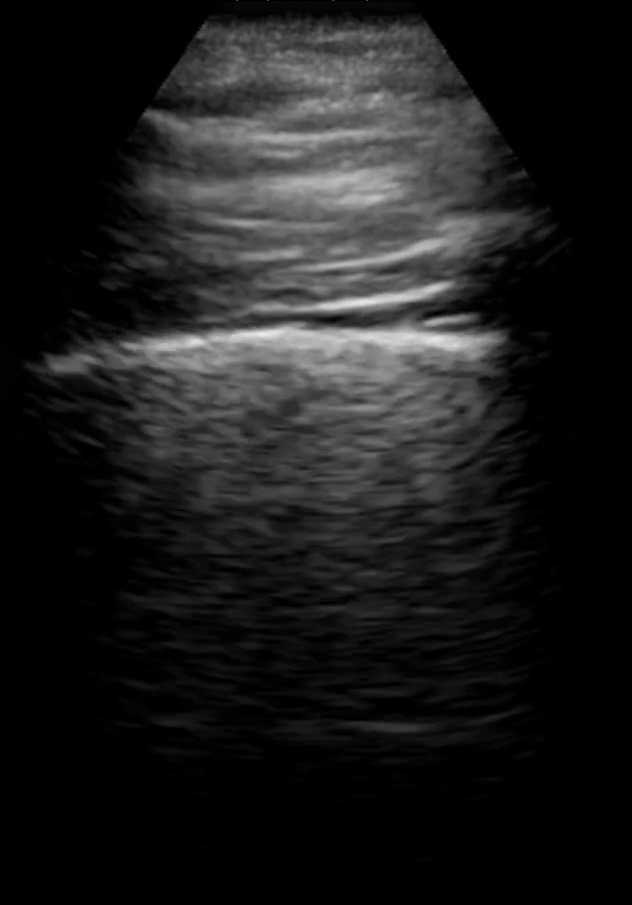
\includegraphics[height=6.5cm]{figuras/short_range.jpg}
	\caption{}
	\end{subfigure}
	\caption{Examples of potential false positives with the proposed approach (a) Presence of organs such as the spleen may be mistaken for B-lines. (b) Short-range images with no B-lines may yield a high total mean brightness.}
	\end{figure}
	
	On the other hand, our representation of videos may not be accurate enough. Although in some cases at least one of the centroids does manage to isolate ocurring B-lines (see figure 5), in others they do not, inducing false negatives. It could be because the B-lines appear very briefly on just a few frames or because of the swinging motion caused by breathing. This could be solved by increasing the number of centroids per video, or by manually selecting the target frames.
	
	A similar approach has been taken with better results by Brattain et al. \cite{brattain}. In their study, pleural lines were removed from the images before evaluating the presence of B-lines, which might facilitate uniformity across the dataset. The duration of the videos was also shorter, with a constant 60 frames per video. Another approach by van Sloun \cite{vanSloun} used deep learning techniques, achieving accuracy of up to $90 \%$.
	

	

% BIBLIOGRAFÍA
\newpage
\newpage
\bibliography{biblio}
\bibliographystyle{plain}

\end{document}
